\documentclass[12pt,letterpaper]{article}
\usepackage[utf8]{inputenc}
\usepackage[english]{babel}
\usepackage{listings}
\usepackage{xcolor}
\usepackage{graphicx}

%For syntax highlighting
\definecolor{codegreen}{rgb}{0,0.6,0}
\definecolor{codegray}{rgb}{0.5,0.5,0.5}
\definecolor{codepurple}{rgb}{0.58,0,0.82}
\definecolor{backcolour}{rgb}{1,1,1}

%%Sets different parameters
\lstdefinestyle{mystyle}{
	backgroundcolor=\color{backcolour},   
    commentstyle=\color{codegreen},
    keywordstyle=\color{magenta},
    numberstyle=\tiny\color{codegray},
    stringstyle=\color{codepurple},
    basicstyle=\ttfamily\footnotesize,
    breakatwhitespace=false,         
    breaklines=true,                 
    captionpos=b,                    
    keepspaces=true,                 
    numbers=left,                    
    numbersep=5pt,                  
    showspaces=false,                
    showstringspaces=false,
    showtabs=false,                  
    tabsize=4
}
\lstset{style=mystyle}

\title{\textbf{Department of Computer Science and Engineering}}
\author{\textbf{S.G.Shivanirudh , 185001146, Semester VI }}

\date{25 February 2021}

\begin{document}
\maketitle
\hrule
\section*{\center{UCS1611 - Internet Programming Lab}}
\hrule 
\bigskip\bigskip

%Assignment name
\section*{\center{\textbf{Ex 03: JavaScript event handling mechanisms, DOM}}}

\subsection*{\underline{\textbf{Patient Registration form}}}
%Objective
\subsection*{\flushleft{Objective:}}
\begin{flushleft}
    Generate a registration form for a hospital to register new patient details.
\end{flushleft}

%Code
\subsection*{\flushleft{Code:}}
\subsubsection*{\flushleft{HTML:}}
\begin{flushleft}
\lstinputlisting[language = HTML]{PatientReg/form.html}
\end{flushleft}

\subsubsection*{{\flushleft{Stylesheet:}}}
\begin{flushleft}
    \lstinputlisting[language = HTML]{PatientReg/style_form.css}
\end{flushleft}

\subsubsection*{{\flushleft{Script file:}}}
\begin{flushleft}
    \lstinputlisting[language = HTML]{PatientReg/script_form.js}
\end{flushleft}

\newpage
%Output
\subsection*{\flushleft{Output:}}
\begin{figure}[h]
    \centering
    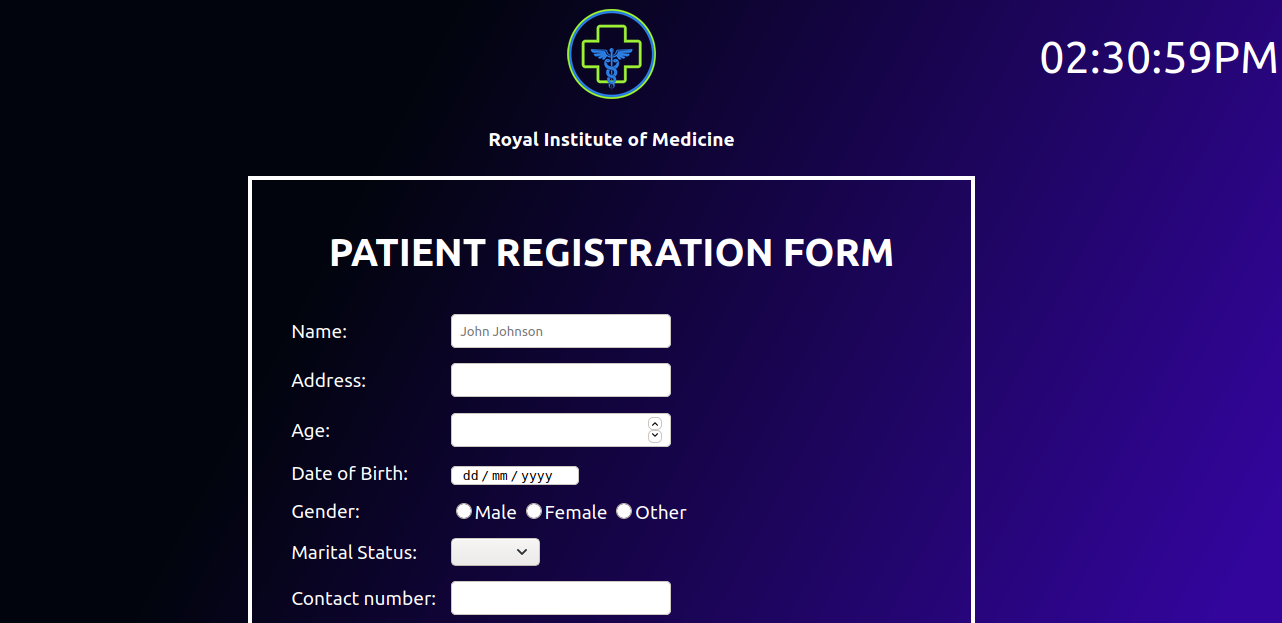
\includegraphics[width = \textwidth]{PatientReg/Pics/form1.png}
\end{figure}
\begin{figure}[h]
    \centering
    
\includegraphics[width = \textwidth]{PatientReg/Pics/form2.png}
\end{figure}
\newpage
\begin{figure}[h!]
    \centering
    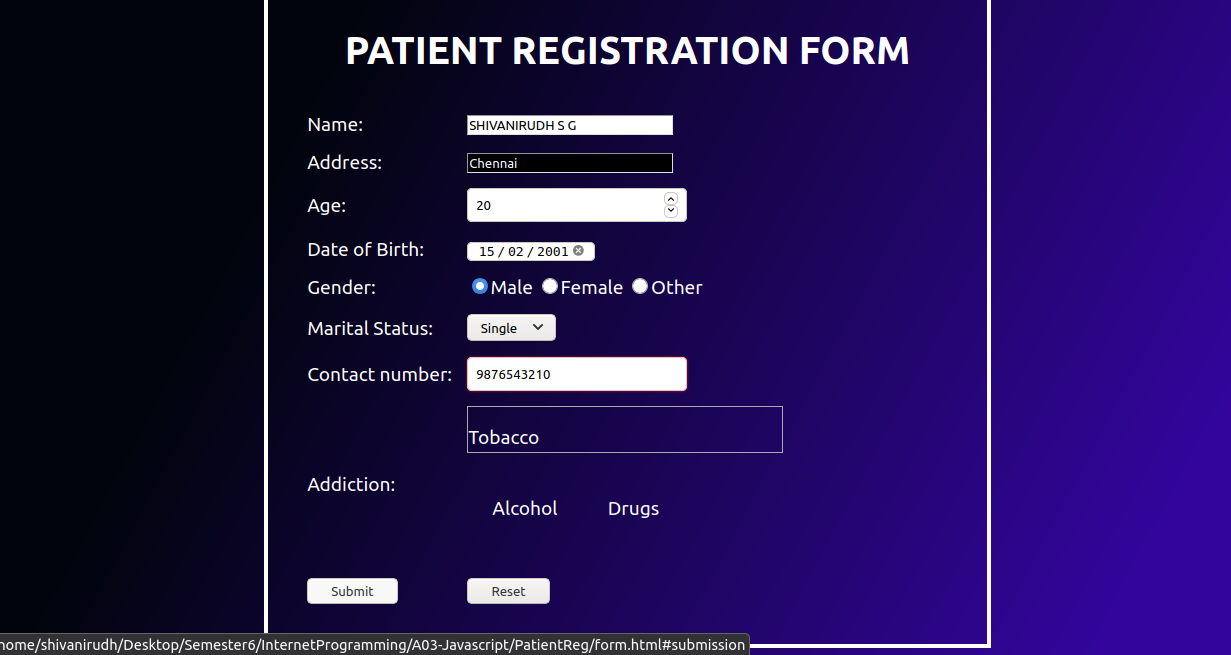
\includegraphics[width = \textwidth]{PatientReg/Pics/form3.png}
\end{figure}
\begin{figure}[h!]
    \centering
    
\includegraphics[width = \textwidth]{PatientReg/Pics/form4.png}
\end{figure}

\hrule
\newpage

\subsection*{\underline{\textbf{Memory Matching Game}}}
%Objective
\subsection*{\flushleft{Objective:}}
\begin{flushleft}
    Write a JS program to develop a memory matching game.
\end{flushleft}

%Code
\subsection*{\flushleft{Code:}}
\subsubsection*{\flushleft{HTML:}}
\begin{flushleft}
\lstinputlisting[language = HTML]{MemoryGame/game.html}
\end{flushleft}

\subsubsection*{{\flushleft{Stylesheet:}}}
\begin{flushleft}
    \lstinputlisting[language = HTML]{MemoryGame/style_game.css}
\end{flushleft}

\subsubsection*{{\flushleft{Script file:}}}
\begin{flushleft}
    \lstinputlisting[language = HTML]{MemoryGame/script_game.js}
\end{flushleft}

\newpage
%Output
\subsection*{\flushleft{Output:}}
\begin{figure}[h]
    \centering
    
\includegraphics[width = \textwidth]{MemoryGame/Pics/game1.png}
\end{figure}
\begin{figure}[h]
    \centering
    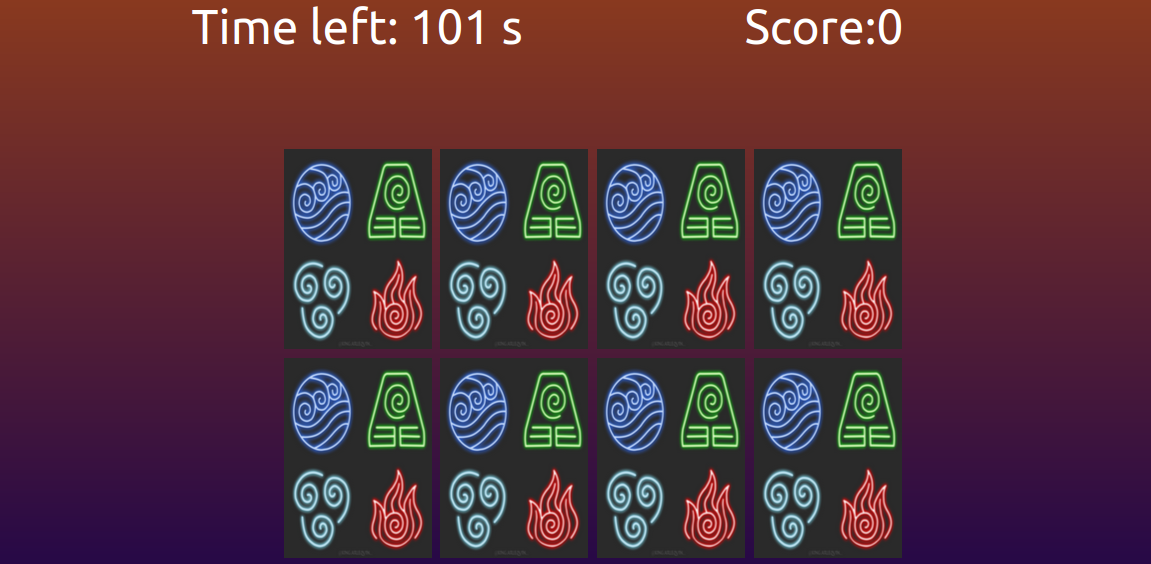
\includegraphics[width = \textwidth]{MemoryGame/Pics/game2.png}
\end{figure}
\newpage
\begin{figure}[h!]
    \centering
    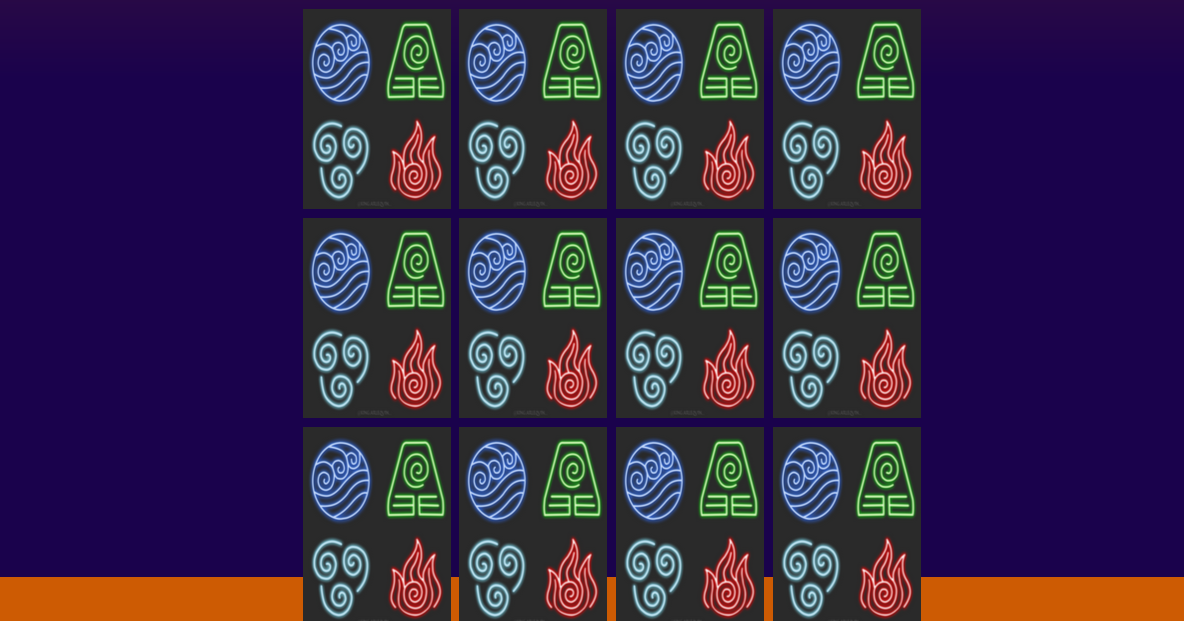
\includegraphics[width = \textwidth]{MemoryGame/Pics/game3.png}
\end{figure}
\begin{figure}[h!]
    \centering
    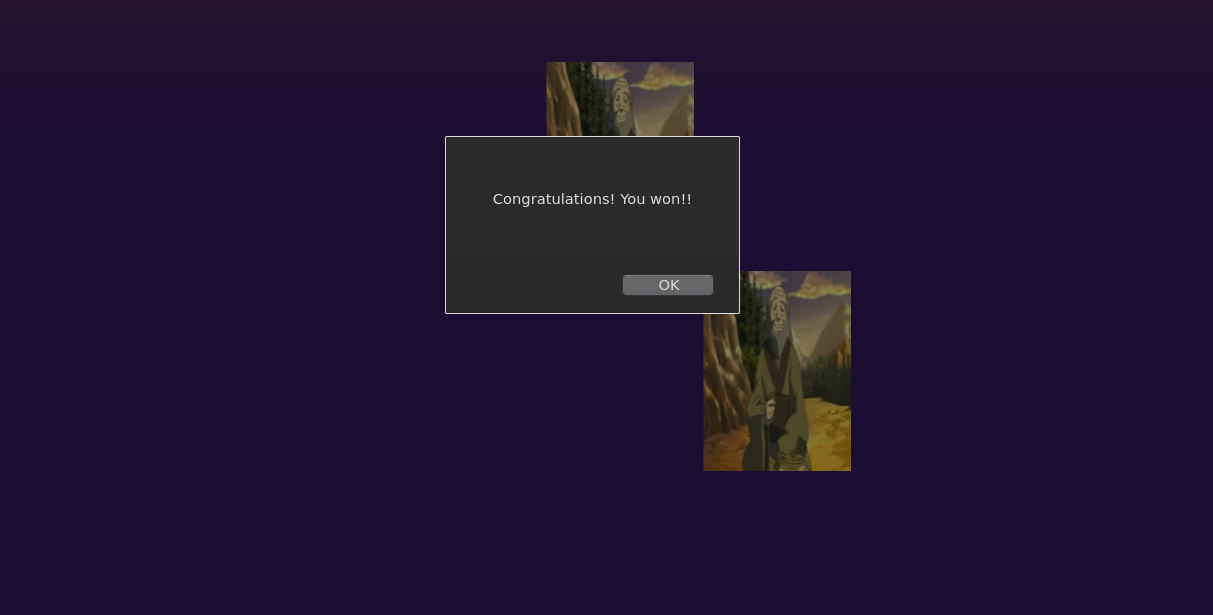
\includegraphics[width = \textwidth]{MemoryGame/Pics/game4.png}
\end{figure}

\hrule

\subsection*{\flushleft{Learning Outcomes:}}
\renewcommand{\labelitemi}{$\textendash$}
\begin{itemize}
    \item Learnt to build a website with HTML5, CSS and JavaScript.
    \item Learnt to use JS scripts to control behaviour of elements.
    \item Learnt to use embedded and external scripts using \textbf{script} tag, and external scripts.
    \item Learnt the different types of events in JS that can be handled and their varied uses.
    \item Learnt to use styling, and behaviour of items using JS.
\end{itemize}
\hrule
\end{document}